%% GENERATED by tools/from_docs.py from stepss-docs. Do not edit by hand:
%% edit the page named below in stepss-docs and regenerate.
%% source: stepss-docs/src/content/docs/models/exciters/ieee-st.md

\chapter{IEEE ST and other exciters}\label{doc:model-exc-ieee-st}

The static (ST) exciters of IEEE Std 421.5, the IEEET5 and SEXS models, and the ENTSO-E simplified exciter.

The \texttt{EXC} sub-record these models are entered with, and the table of IEEE model variants, are on the \hyperref[doc:model-exc]{Exciter Models} page.

\section{ST1A}\label{model-exc-ieee-st:st1a}

The ST1A is a static (thyristor) excitation system with two cascaded lead-lag networks in the voltage regulator path and an inner field current limiter (KLR/ILR). It corresponds to IEEE Std 421.5-2016 Type ST1A. The output limits are proportional to terminal voltage \(V_t\), and field current derating applies through \(K_C\): \(uplim = V_t \cdot V_{RMAX} - K_C \cdot I_{fd}\).

\begin{figure}[htbp]
\centering
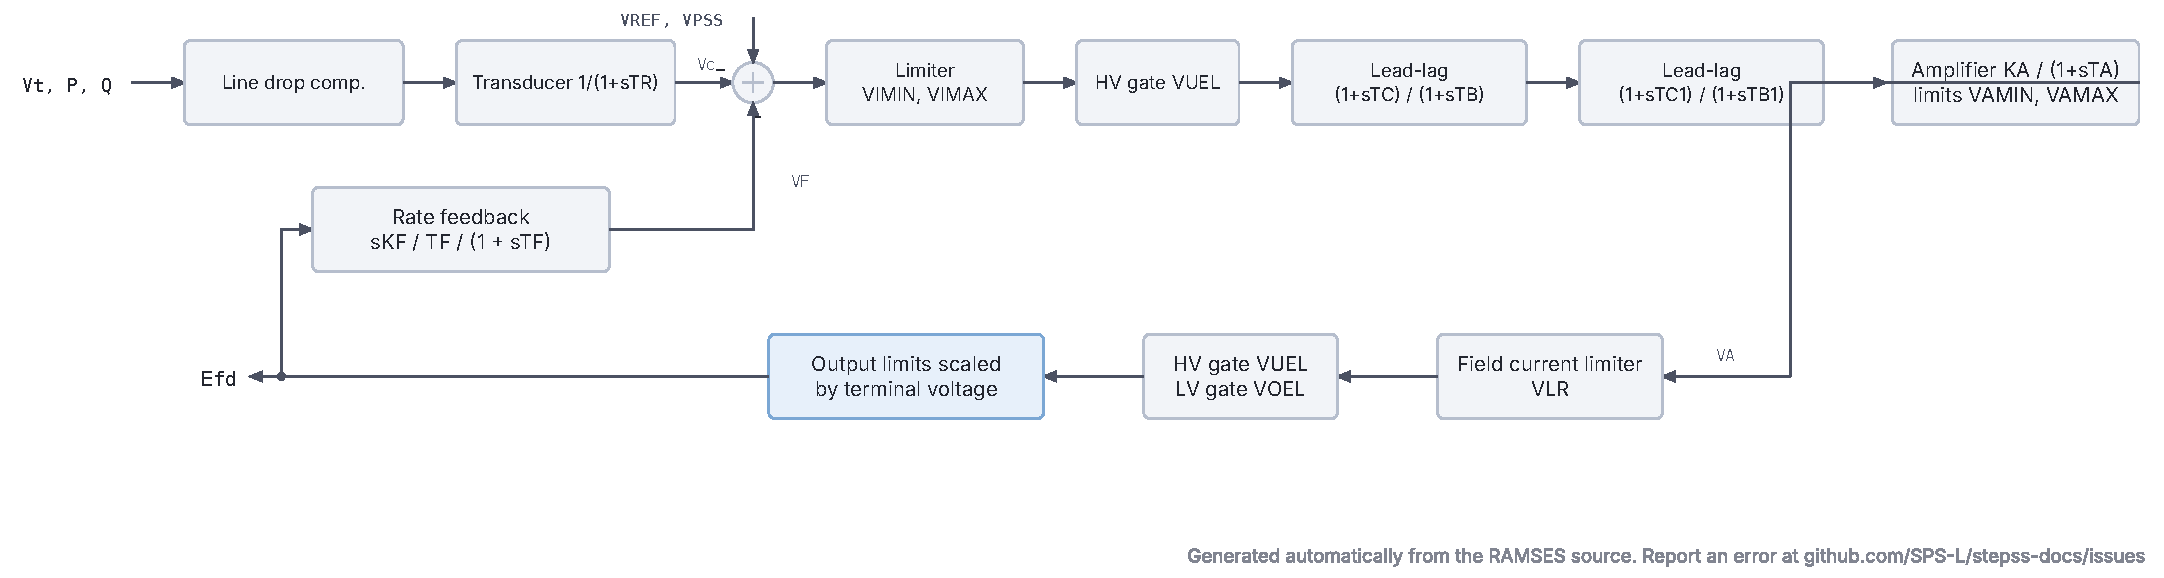
\includegraphics[width=0.98\linewidth]{figures/exc-st1a-light}
\caption{ST1A block diagram.}
\end{figure}

\subsection{Mathematical Description}\label{model-exc-ieee-st:mathematical-description}

The voltage regulator with dual lead-lag and instantaneous field current limiting:

\[\Delta V = V_{REF} - V_c + V_{PSS} + V_{UEL,path} + V_F\]

\[V_1 = \text{clamp}(\Delta V, V_{IMIN}, V_{IMAX})\]

\[V_2(s) = V_1 \cdot \frac{1 + sT_C}{1 + sT_B}\]

\[V_3(s) = V_2 \cdot \frac{1 + sT_{C1}}{1 + sT_{B1}}\]

\[V_A(s) = V_3 \cdot \frac{K_A}{1 + sT_A}, \quad V_{AMIN} \le V_A \le V_{AMAX}\]

Instantaneous field current limiter:

\[V_{LR} = K_{LR}(I_{fd} - I_{LR})\]

\[V_5 = V_A - \max(V_{LR}, 0)\]

Final output with terminal-voltage-dependent limits:

\[E_{fd} = \text{clamp}(V_5, V_t \cdot V_{RMIN}, V_t \cdot V_{RMAX} - K_C \cdot I_{fd})\]

Derivative feedback:

\[V_F(s) = E_{fd} \cdot \frac{sK_F/T_F}{1 + sT_F}\]

\subsection{Signal Flow}\label{model-exc-ieee-st:signal-flow}

\begin{enumerate}
\def\labelenumi{\arabic{enumi}.}
\tightlist
\item
  \textbf{Line drop} (\texttt{algeq}): \(V_{c1}\)
\item
  \textbf{Measurement filter} (\texttt{tf1p}): \(V_c\) with \(T_R\)
\item
  \textbf{AVR summation} (\texttt{algeq}): \(\Delta V\), including UEL (mode 1), PSS, and VF
\item
  \textbf{Error limiter} (\texttt{lim}): \(V_1 \in [V_{IMIN}, V_{IMAX}]\)
\item
  \textbf{UEL gate (mode 2)} (\texttt{max1v1c}): HV gate \(V_2\)
\item
  \textbf{First lead-lag} (\texttt{tf1p1z}): \(V_3\) with \((T_C, T_B)\)
\item
  \textbf{Second lead-lag} (\texttt{tf1p1z}): \(V_4\) with \((T_{C1}, T_{B1})\)
\item
  \textbf{Amplifier} (\texttt{tf1plim}): \(V_A\) with \(K_A\), \(T_A\), \([V_{AMIN}, V_{AMAX}]\)
\item
  \textbf{Field current limiter} (\texttt{algeq}, \texttt{lim}): \(V_{LR}\), \(V_{LRlim}\)
\item
  \textbf{Limiter subtraction} (\texttt{algeq}): \(V_5 = V_A - V_{LRlim}\)
\item
  \textbf{UEL gate (mode 3)} (\texttt{max1v1c}): \(V_6\)
\item
  \textbf{OEL gate} (\texttt{min2v}): \(V_7 = \min(V_6, V_{OEL})\)
\item
  \textbf{Variable-limit output} (\texttt{limvb}): \(E_{fd}\) with terminal-voltage-scaled limits
\item
  \textbf{Derivative feedback} (\texttt{tfder1p}): \(V_F\)
\end{enumerate}

\subsection{Parameters}\label{model-exc-ieee-st:parameters}

\begin{small}\begin{longtable}[]{@{}
  >{\raggedright\arraybackslash}p{(\linewidth - 6\tabcolsep) * \real{0.2133}}
  >{\raggedright\arraybackslash}p{(\linewidth - 6\tabcolsep) * \real{0.5939}}
  >{\raggedright\arraybackslash}p{(\linewidth - 6\tabcolsep) * \real{0.1928}}
@{}}
\toprule\noalign{}
\begin{minipage}[b]{\linewidth}\raggedright
Parameter
\end{minipage} & \begin{minipage}[b]{\linewidth}\raggedright
Description
\end{minipage} & \begin{minipage}[b]{\linewidth}\raggedright
Unit/Type
\end{minipage} \\
\midrule\noalign{}
\endhead
\bottomrule\noalign{}
\endlastfoot
\texttt{Kv} & Voltage compensation gain & pu \\
\texttt{Rc} & Line drop resistance & pu \\
\texttt{Xc} & Line drop reactance & pu \\
\texttt{TR} & Measurement filter time constant & s \\
\texttt{UEL} & UEL connection mode (1=summation, 2=HV gate after V1, 3=HV gate after VA) & integer \\
\texttt{VIMIN} & Input error lower limit & pu \\
\texttt{VIMAX} & Input error upper limit & pu \\
\texttt{VUEL} & UEL signal value & pu \\
\texttt{TC} & First lead-lag numerator & s \\
\texttt{TB} & First lead-lag denominator & s \\
\texttt{TC1} & Second lead-lag numerator & s \\
\texttt{TB1} & Second lead-lag denominator & s \\
\texttt{KA} & Regulator gain & pu \\
\texttt{TA} & Regulator time constant & s \\
\texttt{VAMIN} & Regulator lower limit & pu \\
\texttt{VAMAX} & Regulator upper limit & pu \\
\texttt{VRMIN} & Output lower limit scaling factor & pu \\
\texttt{VRMAX} & Output upper limit scaling factor & pu \\
\texttt{KC} & Field current derating factor & pu \\
\texttt{KF} & Rate feedback gain & pu \\
\texttt{TF} & Rate feedback time constant & s \\
\texttt{KLR} & Field current limiter gain & pu \\
\texttt{ILR} & Field current limiter reference & pu \\
\end{longtable}\end{small}

\subsection{Variants}\label{model-exc-ieee-st:variants}

\begin{small}\begin{longtable}[]{@{}
  >{\raggedright\arraybackslash}p{(\linewidth - 4\tabcolsep) * \real{0.3489}}
  >{\raggedright\arraybackslash}p{(\linewidth - 4\tabcolsep) * \real{0.6511}}
@{}}
\toprule\noalign{}
\begin{minipage}[b]{\linewidth}\raggedright
Model
\end{minipage} & \begin{minipage}[b]{\linewidth}\raggedright
Description
\end{minipage} \\
\midrule\noalign{}
\endhead
\bottomrule\noalign{}
\endlastfoot
\texttt{ST1A} & Base model, IEEE Type ST1A \\
\texttt{ST1A\_IEEEST} & Adds IEEEST single-input PSS (speed or power input, selectable) \\
\texttt{ST1A\_IEEEST\_MAXEX2} & Adds IEEEST PSS + MAXEX2 field current limiter \\
\texttt{ST1A\_PSS2B} & Adds PSS2B dual-input stabilizer \\
\texttt{ST1A\_PSS2B\_MAXEX2} & Adds PSS2B + MAXEX2 \\
\texttt{ST1A\_PSS3B} & Adds PSS3B two-channel second-order filter stabilizer \\
\texttt{ST1A\_PSS4B} & Adds PSS4B three-band stabilizer \\
\texttt{ST1A\_PSS4B\_MAXEX2} & Adds PSS4B + MAXEX2 \\
\texttt{ST1A\_lim} & Integral OEL + stator current limiter (SCL), simplified structure without Kv/Rc/Xc \\
\end{longtable}\end{small}

\subsection{Usage Example}\label{model-exc-ieee-st:usage-example}

\begin{Verbatim}
SYNC_MACH  g1  g1
      # FP FQ P Q: share of the power-flow injection (FP, FQ) or initial power (P in MW, Q in Mvar)
      1.  1.  0.  0.
      # SNOM: Nominal apparent power, used as base power in the machine model (MVA)
      800.
      # Pnom: Nominal active power of the turbine, used as base power for the turbine model (MW)
      760.
      # H: Inertia constant (s)
      3.
      # D: Damping coefficient (usually set to zero when the damper windings are modelled) (pu)
      0.
      # IBRATIO: Field current base ratio I_fB^mac/I_fB^exc (see above) (pu)
      0.95
      # TYPE_MOD: Parameter format keyword: RL or XT (case-insensitive)
      XT
      # Xl: Leakage reactance L_l (pu)
      0.15
      # Xd: d-axis synchronous reactance (pu)
      1.1
      # X'd: d-axis transient reactance (must be smaller than Xd) (pu)
      0.25
      # X"d: d-axis subtransient reactance (pu)
      0.2
      # Xq: q-axis synchronous reactance (pu)
      0.7
      # X'q: q-axis transient reactance (pu)
      *
      # X"q: q-axis subtransient reactance (pu)
      0.2
      # m: Saturation coefficient (set to 0 to neglect saturation)
      0.1
      # n: Saturation exponent (ignored when m = 0)
      6.0257
      # Ra: Armature resistance (pu)
      0.
      # T'do: d-axis open-circuit transient time constant (s)
      5.00
      # T"do: d-axis open-circuit subtransient time constant (s)
      0.05
      # T'qo: q-axis open-circuit transient time constant (s)
      *
      # T"qo: q-axis open-circuit subtransient time constant (s)
      0.1
EXC  ST1A
      # Kv: weight of the terminal voltage in the measured voltage |Kv V + (Rc+jXc) I|; 1 = terminal voltage
      1.
      # Rc: Line drop resistance
      0.
      # Xc: Line drop reactance
      0.
      # TR: Measurement filter time constant
      0.02
      # UEL: UEL connection mode (1=summation, 2=HV gate after V1, 3=HV gate after VA)
      1
      # VIMIN: Input error lower limit
      -0.87
      # VIMAX: Input error upper limit
      0.87
      # VUEL: UEL signal value
      0.0
      # TC: First lead-lag numerator
      1.0
      # TB: First lead-lag denominator
      10.0
      # TC1: Second lead-lag numerator
      0.0
      # TB1: Second lead-lag denominator
      0.0
      # KA: Regulator gain
      200.0
      # TA: Regulator time constant
      0.001
      # VAMIN: Regulator lower limit
      -999.0
      # VAMAX: Regulator upper limit
      999.0
      # VRMIN: Output lower limit scaling factor
      -6.7
      # VRMAX: Output upper limit scaling factor
      7.8
      # KC: Field current derating factor
      0.038
      # KF: Rate feedback gain
      0.0
      # TF: Rate feedback time constant
      1.0
      # KLR: Field current limiter gain
      0.0
      # ILR: Field current limiter reference
      0.0
TOR  CONSTANT
;
\end{Verbatim}

\begin{center}\rule{0.5\linewidth}{0.5pt}\end{center}

\section{ST2A (via EXPIC1)}\label{model-exc-ieee-st:st2a-via-expic1}

The EXPIC1 model implements a static exciter with an AC rotating bus-fed rectifier and an integrating (PI-type) amplifier path: \(K_A(1 + sT_A)/s\). The output \(V_B\) is proportional to the AC voltage phasor magnitude, creating a bus-fed topology analogous to IEEE Type ST2A. When \(K_P = K_I = 0\), the rectifier gain is unity.

\begin{figure}[htbp]
\centering
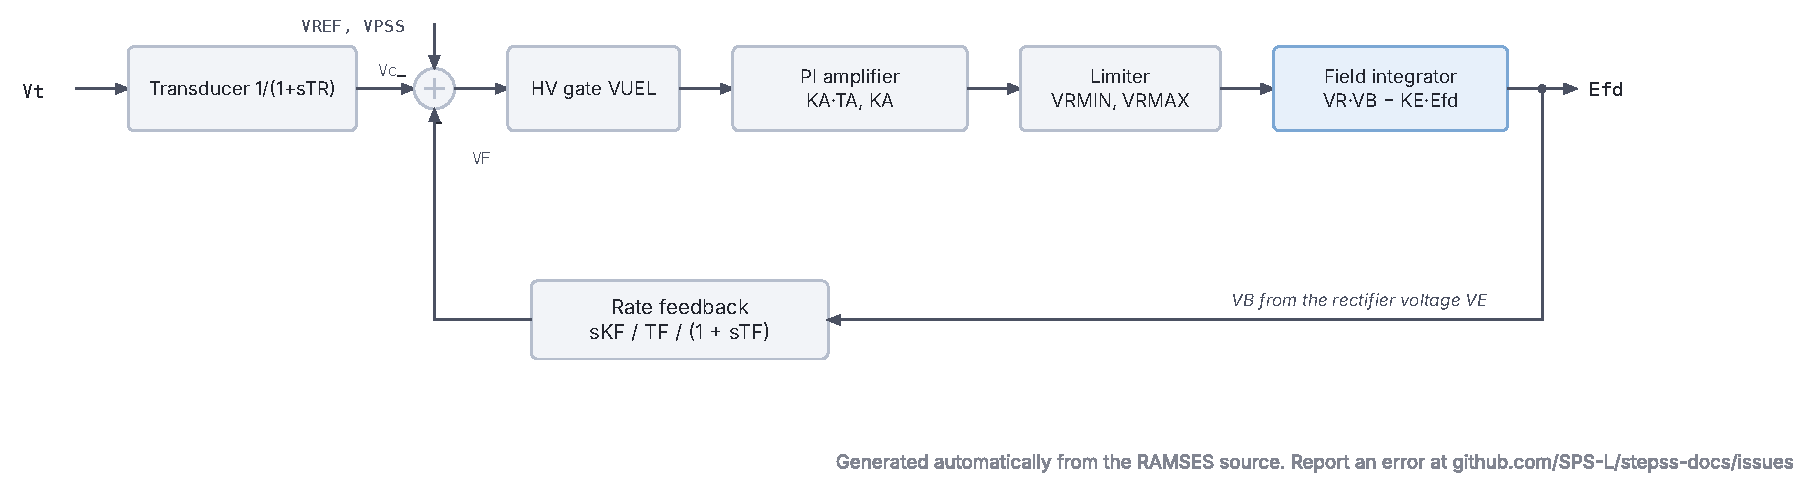
\includegraphics[width=0.98\linewidth]{figures/exc-st2a-light}
\caption{ST2A block diagram.}
\end{figure}

\subsection{Mathematical Description}\label{model-exc-ieee-st:mathematical-description-1}

The AC exciter voltage and rectifier:

\[V_E = |K_P V_t + jK_I V_t|, \quad V_B = V_E \cdot \left(1 - \frac{K_C I_{fd}}{V_E}\right)^+\]

The integrating amplifier:

\[G_{amp}(s) = K_A \cdot \frac{1 + sT_A}{s}\]

The field voltage integrator:

\[\dot{E}_{fd} = \frac{1}{T_E}\left[V_R \cdot V_B - K_E \cdot E_{fd}\right], \quad E_{FDMIN} \le E_{fd} \le E_{FDMAX}\]

\subsection{Signal Flow}\label{model-exc-ieee-st:signal-flow-1}

\begin{enumerate}
\def\labelenumi{\arabic{enumi}.}
\tightlist
\item
  \textbf{Voltage measurement} (\texttt{tf1p}): \(V_c\) with \(T_R\)
\item
  \textbf{Summation} (\texttt{algeq}): \(\Delta V = V_{REF} - V_c - V_F - \Delta V_{PSS}\)
\item
  \textbf{UEL gate} (\texttt{max1v1c}): clamped to \(V_{UEL}\)
\item
  \textbf{PI amplifier} (\texttt{pictl}): \(V_A\) with \(K_{gain} = K_A \cdot T_A\) and \(K_A\)
\item
  \textbf{Output limiter} (\texttt{lim}): \(V_R \in [V_{RMIN}, V_{RMAX}]\)
\item
  \textbf{Rectifier voltage} (\texttt{algeq}): \(V_E\), \(V_B\)
\item
  \textbf{Field integrator} (\texttt{inlim}): \(E_{fd}\) from \(V_R \cdot V_B - K_E \cdot E_{fd}\)
\item
  \textbf{Derivative feedback} (\texttt{tfder1p}): \(V_F\)
\end{enumerate}

\subsection{Parameters}\label{model-exc-ieee-st:parameters-1}

\begin{small}\begin{longtable}[]{@{}lll@{}}
\toprule\noalign{}
Parameter & Description & Unit/Type \\
\midrule\noalign{}
\endhead
\bottomrule\noalign{}
\endlastfoot
\texttt{Kvcomp} & Voltage compensation gain & pu \\
\texttt{Rc} & Line drop resistance & pu \\
\texttt{Xc} & Line drop reactance & pu \\
\texttt{TR} & Measurement time constant & s \\
\texttt{VUEL} & UEL signal & pu \\
\texttt{KA} & Amplifier gain & pu \\
\texttt{TA} & Amplifier time constant & s \\
\texttt{VRMAX} & Maximum regulator output & pu \\
\texttt{VRMIN} & Minimum regulator output & pu \\
\texttt{KF} & Rate feedback gain & pu \\
\texttt{TF} & Rate feedback time constant & s \\
\texttt{KE} & Exciter self-excitation constant & pu \\
\texttt{EFDMAX} & Maximum field voltage & pu \\
\texttt{EFDMIN} & Minimum field voltage & pu \\
\texttt{TE} & Field integrator time constant & s \\
\texttt{KP} & AC source voltage proportional factor & pu \\
\texttt{KI} & AC source voltage quadrature factor & pu \\
\texttt{KC} & Commutation voltage drop factor & pu \\
\end{longtable}\end{small}

\subsection{Variants}\label{model-exc-ieee-st:variants-1}

\begin{small}\begin{longtable}[]{@{}ll@{}}
\toprule\noalign{}
Model & Description \\
\midrule\noalign{}
\endhead
\bottomrule\noalign{}
\endlastfoot
\texttt{EXPIC1} & Base bus-fed static exciter \\
\texttt{EXPIC1\_PSS2B} & Adds PSS2B dual-input stabilizer \\
\texttt{EXPIC1\_PSS2B\_MAXEX2} & Adds PSS2B + MAXEX2 field current limiter \\
\end{longtable}\end{small}

\subsection{Usage Example}\label{model-exc-ieee-st:usage-example-1}

\begin{Verbatim}
SYNC_MACH  g1  g1
      # FP FQ P Q: share of the power-flow injection (FP, FQ) or initial power (P in MW, Q in Mvar)
      1.  1.  0.  0.
      # SNOM: Nominal apparent power, used as base power in the machine model (MVA)
      800.
      # Pnom: Nominal active power of the turbine, used as base power for the turbine model (MW)
      760.
      # H: Inertia constant (s)
      3.
      # D: Damping coefficient (usually set to zero when the damper windings are modelled) (pu)
      0.
      # IBRATIO: Field current base ratio I_fB^mac/I_fB^exc (see above) (pu)
      0.95
      # TYPE_MOD: Parameter format keyword: RL or XT (case-insensitive)
      XT
      # Xl: Leakage reactance L_l (pu)
      0.15
      # Xd: d-axis synchronous reactance (pu)
      1.1
      # X'd: d-axis transient reactance (must be smaller than Xd) (pu)
      0.25
      # X"d: d-axis subtransient reactance (pu)
      0.2
      # Xq: q-axis synchronous reactance (pu)
      0.7
      # X'q: q-axis transient reactance (pu)
      *
      # X"q: q-axis subtransient reactance (pu)
      0.2
      # m: Saturation coefficient (set to 0 to neglect saturation)
      0.1
      # n: Saturation exponent (ignored when m = 0)
      6.0257
      # Ra: Armature resistance (pu)
      0.
      # T'do: d-axis open-circuit transient time constant (s)
      5.00
      # T"do: d-axis open-circuit subtransient time constant (s)
      0.05
      # T'qo: q-axis open-circuit transient time constant (s)
      *
      # T"qo: q-axis open-circuit subtransient time constant (s)
      0.1
EXC  EXPIC1
      # Kvcomp: weight of the terminal voltage in the measured voltage |Kv V + (Rc+jXc) I|; 1 = terminal voltage
      1.
      # Rc: Compensation resistance (pu)
      0.
      # Xc: Compensation reactance (pu)
      0.
      # TR: Voltage measurement time constant (s)
      0.02
      # VUEL: UEL signal, lower bound of the voltage error (pu)
      -99999
      # KA: PI amplifier integral gain, KA(1+sTA)/s (1/s)
      200.0
      # TA: PI amplifier time constant (s)
      0.02
      # VRMAX: Maximum regulator output (pu)
      99.0
      # VRMIN: Minimum regulator output (pu)
      -99.0
      # KF: Rate feedback gain (pu)
      0.0
      # TF: Rate feedback time constant (s)
      1.0
      # KE: Exciter self-excitation constant (pu)
      1.0
      # EFDMAX: Maximum field voltage (pu)
      8.0
      # EFDMIN: Minimum field voltage (pu)
      -8.0
      # TE: Field integrator time constant (s)
      0.5
      # KP: Potential source gain on terminal voltage (pu)
      0.0
      # KI: Current source gain on terminal current (pu)
      1.0
      # KC: Rectifier commutation factor (pu)
      0.0
TOR  CONSTANT
;
\end{Verbatim}

\begin{center}\rule{0.5\linewidth}{0.5pt}\end{center}

\section{IEEET5}\label{model-exc-ieee-st:ieeet5}

The IEEET5 (also referenced as DC5A in some conventions) is a non-continuously acting exciter similar to DC3A but uses an inner limiter block \texttt{lim\_civ} that gates the integrator holding signal within a deadband \(\pm K_V\). This creates the three-state (hold/raise/lower) behavior of rheostatic controllers.

\begin{figure}[htbp]
\centering
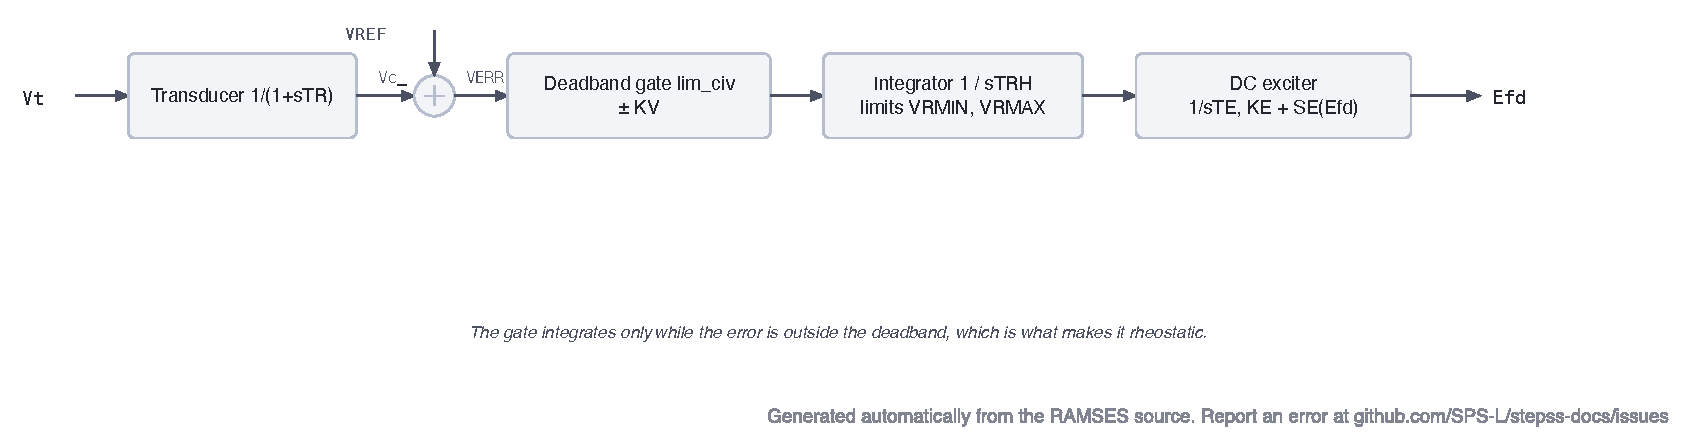
\includegraphics[width=0.98\linewidth]{figures/exc-ieeet5-light}
\caption{IEEET5 block diagram.}
\end{figure}

\subsection{Mathematical Description}\label{model-exc-ieee-st:mathematical-description-2}

\[V_{ERR} = V_{REF} - V_c\]

The integrator for rheostat position:

\[\dot{V}_{RH} = \frac{1}{T_{RH}} \cdot V_{ERR}, \quad V_{RMIN} \le V_{RH} \le V_{RMAX}\]

The \texttt{lim\_civ} block implements the deadband gating so that integration is active only when \(|V_{ERR}| > K_V\):

\[V_R = \begin{cases} V_{RMIN} & V_{ERR} < -K_V \\ V_{RH} & |V_{ERR}| \le K_V \\ V_{RMAX} & V_{ERR} > K_V \end{cases}\]

\[\dot{E}_{fd} = \frac{1}{T_E}\left[V_R - \left(K_E + S_E(E_{fd})\right) E_{fd}\right]\]

\subsection{Parameters}\label{model-exc-ieee-st:parameters-2}

\begin{small}\begin{longtable}[]{@{}lll@{}}
\toprule\noalign{}
Parameter & Description & Unit/Type \\
\midrule\noalign{}
\endhead
\bottomrule\noalign{}
\endlastfoot
\texttt{Kvcomp} & Voltage compensation gain & pu \\
\texttt{Rc} & Line drop resistance & pu \\
\texttt{Xc} & Line drop reactance & pu \\
\texttt{TRH} & Rheostat time & s \\
\texttt{KV} & Controller sensitivity deadband & pu \\
\texttt{VRMAX} & Maximum field voltage & pu \\
\texttt{VRMIN} & Minimum field voltage & pu \\
\texttt{TE} & Exciter integrator time constant & s \\
\texttt{KE} & Exciter self-excitation constant & pu \\
\texttt{E1} & Saturation point 1 & pu \\
\texttt{SE1} & Saturation factor at \(E_1\) & pu \\
\texttt{E2} & Saturation point 2 & pu \\
\texttt{SE2} & Saturation factor at \(E_2\) & pu \\
\end{longtable}\end{small}

\subsection{Variants}\label{model-exc-ieee-st:variants-2}

\begin{small}\begin{longtable}[]{@{}ll@{}}
\toprule\noalign{}
Model & Description \\
\midrule\noalign{}
\endhead
\bottomrule\noalign{}
\endlastfoot
\texttt{IEEET5} & Base model, non-continuously acting DC exciter \\
\end{longtable}\end{small}

\begin{center}\rule{0.5\linewidth}{0.5pt}\end{center}

\section{SEXS}\label{model-exc-ieee-st:sexs}

The SEXS (Simplified Excitation System) is a minimal two-parameter static exciter model from CIGR\'E publications, widely used for cases where detailed exciter data is unavailable. It has no measurement filter, no line drop compensation, and no rate feedback, just a lead-lag network and a limited first-order block.

\begin{figure}[htbp]
\centering
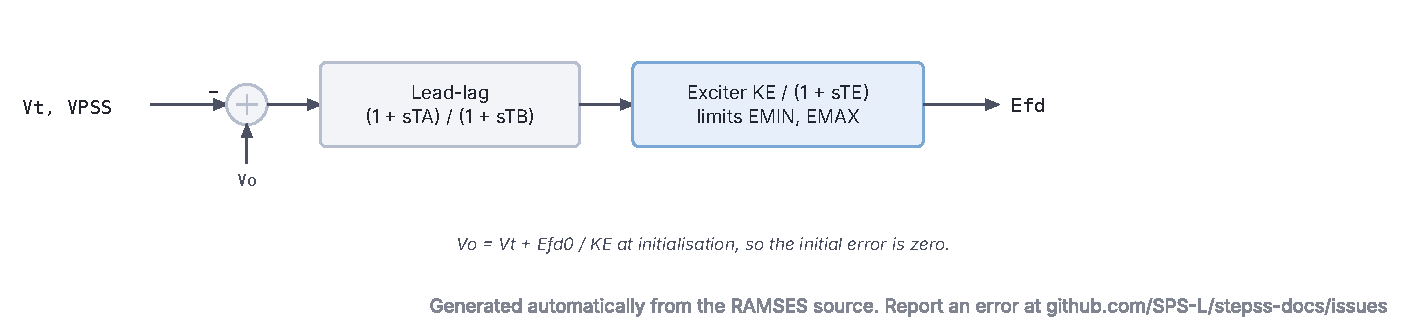
\includegraphics[width=0.98\linewidth]{figures/exc-sexs-light}
\caption{SEXS block diagram.}
\end{figure}

\subsection{Mathematical Description}\label{model-exc-ieee-st:mathematical-description-3}

\[\Delta V_{AVR} = V_t - V_o + V_{PSS}\]

\[G_{lag}(s) = \frac{1 + sT_A}{1 + sT_B}\]

\[E_{fd}(s) = G_{lag}(\Delta V_{AVR}) \cdot \frac{K_E}{1 + sT_E}, \quad E_{MIN} \le E_{fd} \le E_{MAX}\]

where \(V_o = V_t + E_{fd,0}/K_E\) is computed from initial conditions to achieve zero initial error.

\subsection{Parameters}\label{model-exc-ieee-st:parameters-3}

\begin{small}\begin{longtable}[]{@{}lll@{}}
\toprule\noalign{}
Parameter & Description & Unit/Type \\
\midrule\noalign{}
\endhead
\bottomrule\noalign{}
\endlastfoot
\texttt{TA} & Lead-lag numerator time constant & s \\
\texttt{TB} & Lead-lag denominator time constant & s \\
\texttt{KE} & Exciter gain & pu \\
\texttt{TE} & Exciter time constant & s \\
\texttt{EMIN} & Minimum field voltage & pu \\
\texttt{EMAX} & Maximum field voltage & pu \\
\end{longtable}\end{small}

\subsection{Variants}\label{model-exc-ieee-st:variants-3}

\begin{small}\begin{longtable}[]{@{}
  >{\raggedright\arraybackslash}p{(\linewidth - 4\tabcolsep) * \real{0.3350}}
  >{\raggedright\arraybackslash}p{(\linewidth - 4\tabcolsep) * \real{0.6650}}
@{}}
\toprule\noalign{}
\begin{minipage}[b]{\linewidth}\raggedright
Model
\end{minipage} & \begin{minipage}[b]{\linewidth}\raggedright
Description
\end{minipage} \\
\midrule\noalign{}
\endhead
\bottomrule\noalign{}
\endlastfoot
\texttt{SEXS} & Base simplified exciter \\
\texttt{SEXS\_IEEEST} & Adds IEEEST PSS (multi-mode: speed, power, or accelerating power input) \\
\texttt{SEXS\_STAB3\_lim} & Adds STAB3 PSS + integral OEL \\
\end{longtable}\end{small}

\subsection{Usage Example}\label{model-exc-ieee-st:usage-example-2}

\begin{Verbatim}
SYNC_MACH  g1  g1
      # FP FQ P Q: share of the power-flow injection (FP, FQ) or initial power (P in MW, Q in Mvar)
      1.  1.  0.  0.
      # SNOM: Nominal apparent power, used as base power in the machine model (MVA)
      800.
      # Pnom: Nominal active power of the turbine, used as base power for the turbine model (MW)
      760.
      # H: Inertia constant (s)
      3.
      # D: Damping coefficient (usually set to zero when the damper windings are modelled) (pu)
      0.
      # IBRATIO: Field current base ratio I_fB^mac/I_fB^exc (see above) (pu)
      0.95
      # TYPE_MOD: Parameter format keyword: RL or XT (case-insensitive)
      XT
      # Xl: Leakage reactance L_l (pu)
      0.15
      # Xd: d-axis synchronous reactance (pu)
      1.1
      # X'd: d-axis transient reactance (must be smaller than Xd) (pu)
      0.25
      # X"d: d-axis subtransient reactance (pu)
      0.2
      # Xq: q-axis synchronous reactance (pu)
      0.7
      # X'q: q-axis transient reactance (pu)
      *
      # X"q: q-axis subtransient reactance (pu)
      0.2
      # m: Saturation coefficient (set to 0 to neglect saturation)
      0.1
      # n: Saturation exponent (ignored when m = 0)
      6.0257
      # Ra: Armature resistance (pu)
      0.
      # T'do: d-axis open-circuit transient time constant (s)
      5.00
      # T"do: d-axis open-circuit subtransient time constant (s)
      0.05
      # T'qo: q-axis open-circuit transient time constant (s)
      *
      # T"qo: q-axis open-circuit subtransient time constant (s)
      0.1
EXC  SEXS
      # TA: Lead-lag numerator time constant
      0.1
      # TB: Lead-lag denominator time constant
      10.0
      # KE: Exciter gain
      25.0
      # TE: Exciter time constant
      0.5
      # EMIN: Minimum field voltage
      -5.0
      # EMAX: Maximum field voltage
      5.0
TOR  CONSTANT
;
\end{Verbatim}

\begin{center}\rule{0.5\linewidth}{0.5pt}\end{center}

\section{ENTSOE\_simp}\label{model-exc-ieee-st:entsoe_simp}

The ENTSO-E simplified exciter combines a built-in speed-signal PSS with a simple lead-lag AVR and first-order exciter block. It is the standard ENTSO-E model for dynamic studies where detailed exciter data is unavailable.

\begin{figure}[htbp]
\centering
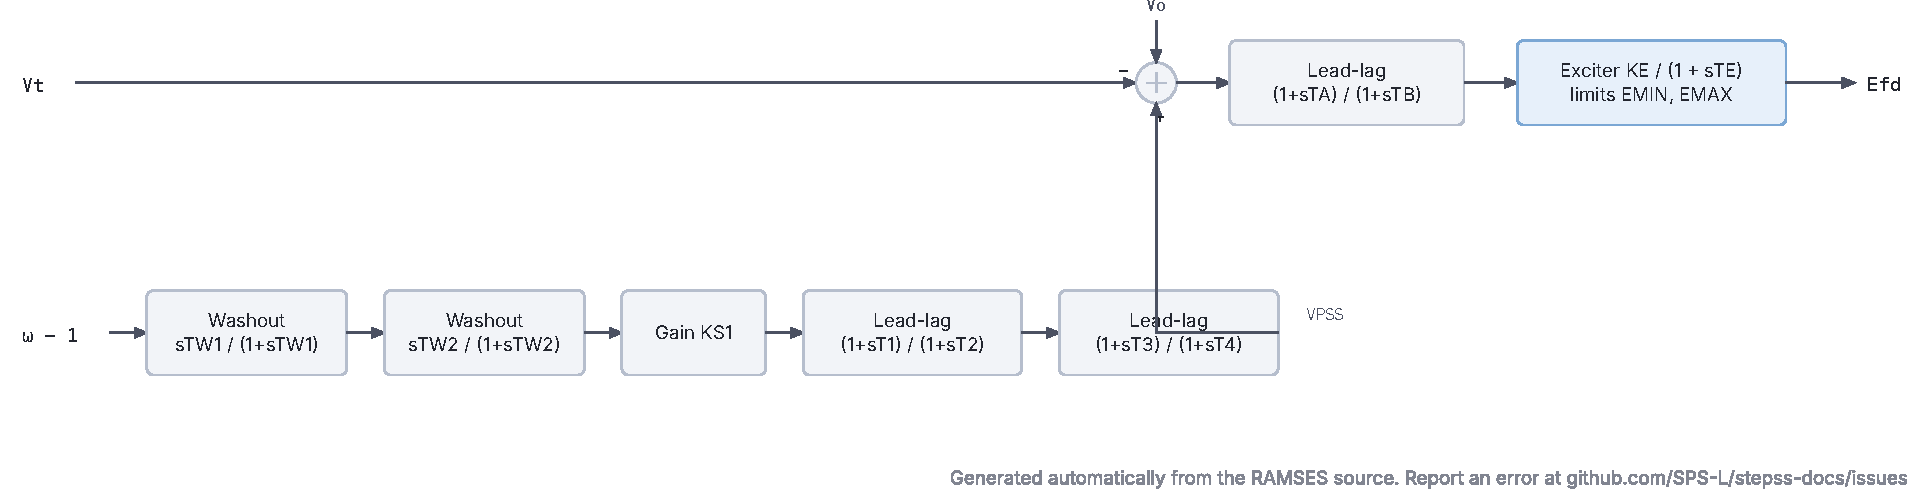
\includegraphics[width=0.98\linewidth]{figures/exc-entsoe-simp-light}
\caption{ENTSOE\_simp block diagram.}
\end{figure}

\subsection{Mathematical Description}\label{model-exc-ieee-st:mathematical-description-4}

The PSS (speed input \(\omega - 1\)) uses two washout stages and two lead-lag stages:

\[V_{PSS}(s) = (\omega - 1) \cdot \frac{sT_{W1}}{1+sT_{W1}} \cdot \frac{sT_{W2}}{1+sT_{W2}} \cdot K_{S1} \cdot \frac{1+sT_1}{1+sT_2} \cdot \frac{1+sT_3}{1+sT_4}\]

The AVR:

\[\Delta V_{AVR} = V_t - V_o + V_{PSS}\]

\[G_{lag}(s) = \frac{1 + sT_A}{1 + sT_B}\]

\[E_{fd}(s) = G_{lag}(\Delta V_{AVR}) \cdot \frac{K_E}{1 + sT_E}, \quad E_{MIN} \le E_{fd} \le E_{MAX}\]

\subsection{Parameters}\label{model-exc-ieee-st:parameters-4}

\begin{small}\begin{longtable}[]{@{}lll@{}}
\toprule\noalign{}
Parameter & Description & Unit/Type \\
\midrule\noalign{}
\endhead
\bottomrule\noalign{}
\endlastfoot
\texttt{TW1} & First washout time constant & s \\
\texttt{TW2} & Second washout time constant & s \\
\texttt{KS1} & PSS gain & pu \\
\texttt{T1} & First lead-lag numerator & s \\
\texttt{T2} & First lead-lag denominator & s \\
\texttt{T3} & Second lead-lag numerator & s \\
\texttt{T4} & Second lead-lag denominator & s \\
\texttt{VSTMIN} & PSS output lower limit & pu \\
\texttt{VSTMAX} & PSS output upper limit & pu \\
\texttt{TA} & AVR lead-lag numerator & s \\
\texttt{TB} & AVR lead-lag denominator & s \\
\texttt{KE} & Exciter gain & pu \\
\texttt{TE} & Exciter time constant & s \\
\texttt{EMIN} & Minimum field voltage & pu \\
\texttt{EMAX} & Maximum field voltage & pu \\
\end{longtable}\end{small}

\subsection{Variants}\label{model-exc-ieee-st:variants-4}

\begin{small}\begin{longtable}[]{@{}ll@{}}
\toprule\noalign{}
Model & Description \\
\midrule\noalign{}
\endhead
\bottomrule\noalign{}
\endlastfoot
\texttt{ENTSOE\_simp} & Base ENTSO-E simplified model with integrated PSS \\
\texttt{ENTSOE\_lim} & Adds integral OEL (same structure as \texttt{AC8B\_lim} OEL) \\
\end{longtable}\end{small}

\subsection{Usage Example}\label{model-exc-ieee-st:usage-example-3}

\begin{Verbatim}
SYNC_MACH  g1  g1
      # FP FQ P Q: share of the power-flow injection (FP, FQ) or initial power (P in MW, Q in Mvar)
      1.  1.  0.  0.
      # SNOM: Nominal apparent power, used as base power in the machine model (MVA)
      800.
      # Pnom: Nominal active power of the turbine, used as base power for the turbine model (MW)
      760.
      # H: Inertia constant (s)
      3.
      # D: Damping coefficient (usually set to zero when the damper windings are modelled) (pu)
      0.
      # IBRATIO: Field current base ratio I_fB^mac/I_fB^exc (see above) (pu)
      0.95
      # TYPE_MOD: Parameter format keyword: RL or XT (case-insensitive)
      XT
      # Xl: Leakage reactance L_l (pu)
      0.15
      # Xd: d-axis synchronous reactance (pu)
      1.1
      # X'd: d-axis transient reactance (must be smaller than Xd) (pu)
      0.25
      # X"d: d-axis subtransient reactance (pu)
      0.2
      # Xq: q-axis synchronous reactance (pu)
      0.7
      # X'q: q-axis transient reactance (pu)
      *
      # X"q: q-axis subtransient reactance (pu)
      0.2
      # m: Saturation coefficient (set to 0 to neglect saturation)
      0.1
      # n: Saturation exponent (ignored when m = 0)
      6.0257
      # Ra: Armature resistance (pu)
      0.
      # T'do: d-axis open-circuit transient time constant (s)
      5.00
      # T"do: d-axis open-circuit subtransient time constant (s)
      0.05
      # T'qo: q-axis open-circuit transient time constant (s)
      *
      # T"qo: q-axis open-circuit subtransient time constant (s)
      0.1
EXC  ENTSOE_simp
      # TW1: First PSS washout time constant (s)
      10.0
      # TW2: Second PSS washout time constant (s)
      3.0
      # KS1: PSS gain, applied in the first lead-lag (pu/pu)
      10.0
      # T1: PSS first lead-lag numerator time constant (s)
      0.2
      # T2: PSS first lead-lag denominator time constant (s)
      0.1
      # T3: PSS second lead-lag numerator time constant (s)
      0.1
      # T4: PSS second lead-lag denominator time constant (s)
      0.1
      # VSTMIN: PSS output lower limit (pu)
      -0.05
      # VSTMAX: PSS output upper limit (pu)
      0.05
      # TA: AVR lead-lag numerator time constant (s)
      0.05
      # TB: AVR lead-lag denominator time constant (s)
      0.1
      # KE: Exciter gain (pu/pu)
      25.0
      # TE: Exciter time constant (s)
      1.0
      # EMIN: Minimum field voltage (pu)
      -10.0
      # EMAX: Maximum field voltage (pu)
      10.0
TOR  CONSTANT
;
\end{Verbatim}
